\documentclass[12pt, letterpaper, twoside]{article}
%%%%%%%%%%%%%%%%%%%%%%%%
% Imports
%%%%%%%%%%%%%%%%%%%%%%%%
\usepackage[utf8]{inputenc}
\usepackage[acronyms]{glossaries}
\usepackage{graphicx}
\usepackage{biblatex}

%%%%%%%%%%%%%%%%%%%%%%%%
% Metadata
%%%%%%%%%%%%%%%%%%%%%%%%
\title{EWT summary}
\author{Ernesto Casablanca}
\date{\today}
\graphicspath{ {./img/} }

%%%%%%%%%%%%%%%%%%%%%%%%
% Glossary
%%%%%%%%%%%%%%%%%%%%%%%%
% \makeglossaries
\newacronym{did}{DID}{Decentralized IDentifiers}
\newacronym{der}{DER}{Distributed Energy Resource}
\newacronym{dsm}{DSM}{Demand Side Management}
\newacronym{irec}{I-REC}{International Renewable Energy Certificate}
\newacronym{poa}{PoA}{Proof of Authority}
\newacronym{pos}{PoS}{Proof of Stake}
\newacronym{evm}{EVM}{Ethereum Virtual Machine}
\newacronym{erc}{ERC}{Ethereum Request for Comment}
\newacronym{ewns}{EWNS}{Energy Web Name Service}
\newacronym{ewc}{EWC}{Energy Web Chain}
\newacronym{eac}{EAC}{Rnergy Attribute Certificate}
\newacronym{kms}{KMS}{Key Management Sysyem}
\newacronym{spf}{SPO}{Single Point of Failure}
\newacronym{ipfs}{IPFS}{InterPlanetary File System}
\newacronym{dht}{DHT}{Distributed Hash Tables}
\newacronym{sla}{SLA}{Service-Level Agreement}

%%%%%%%%%%%%%%%%%%%%%%%%
% References
%%%%%%%%%%%%%%%%%%%%%%%%
\addbibresource{resources.bib} %Import the bibliography file

%%%%%%%%%%%%%%%%%%%%%%%%
% Init document
%%%%%%%%%%%%%%%%%%%%%%%%
\begin{document}

% \begin{titlepage}
%     \maketitle
% \end{titlepage}

\tableofcontents

\newpage

\begin{abstract}
    Breve introduzione alla \gls{ewc}, la blockchain utilizzata da Energy Web
\end{abstract}

\section{Implementazione}
Il cuore del progetto di Energy Web è EW-DOS, un'infrastruttura open-source, pubblica e digitale.
L'intero sistema è costituito da tre macro componenti, ognuno con uno scopo specifico:

\begin{itemize}
    \item Trust - \gls{ewc}
    \item Utility - Servizi e astrazioni sopra la blockchain
    \item Toolkit - Frameworks per la costruzione di applicazioni
\end{itemize}

\begin{figure}[h]
    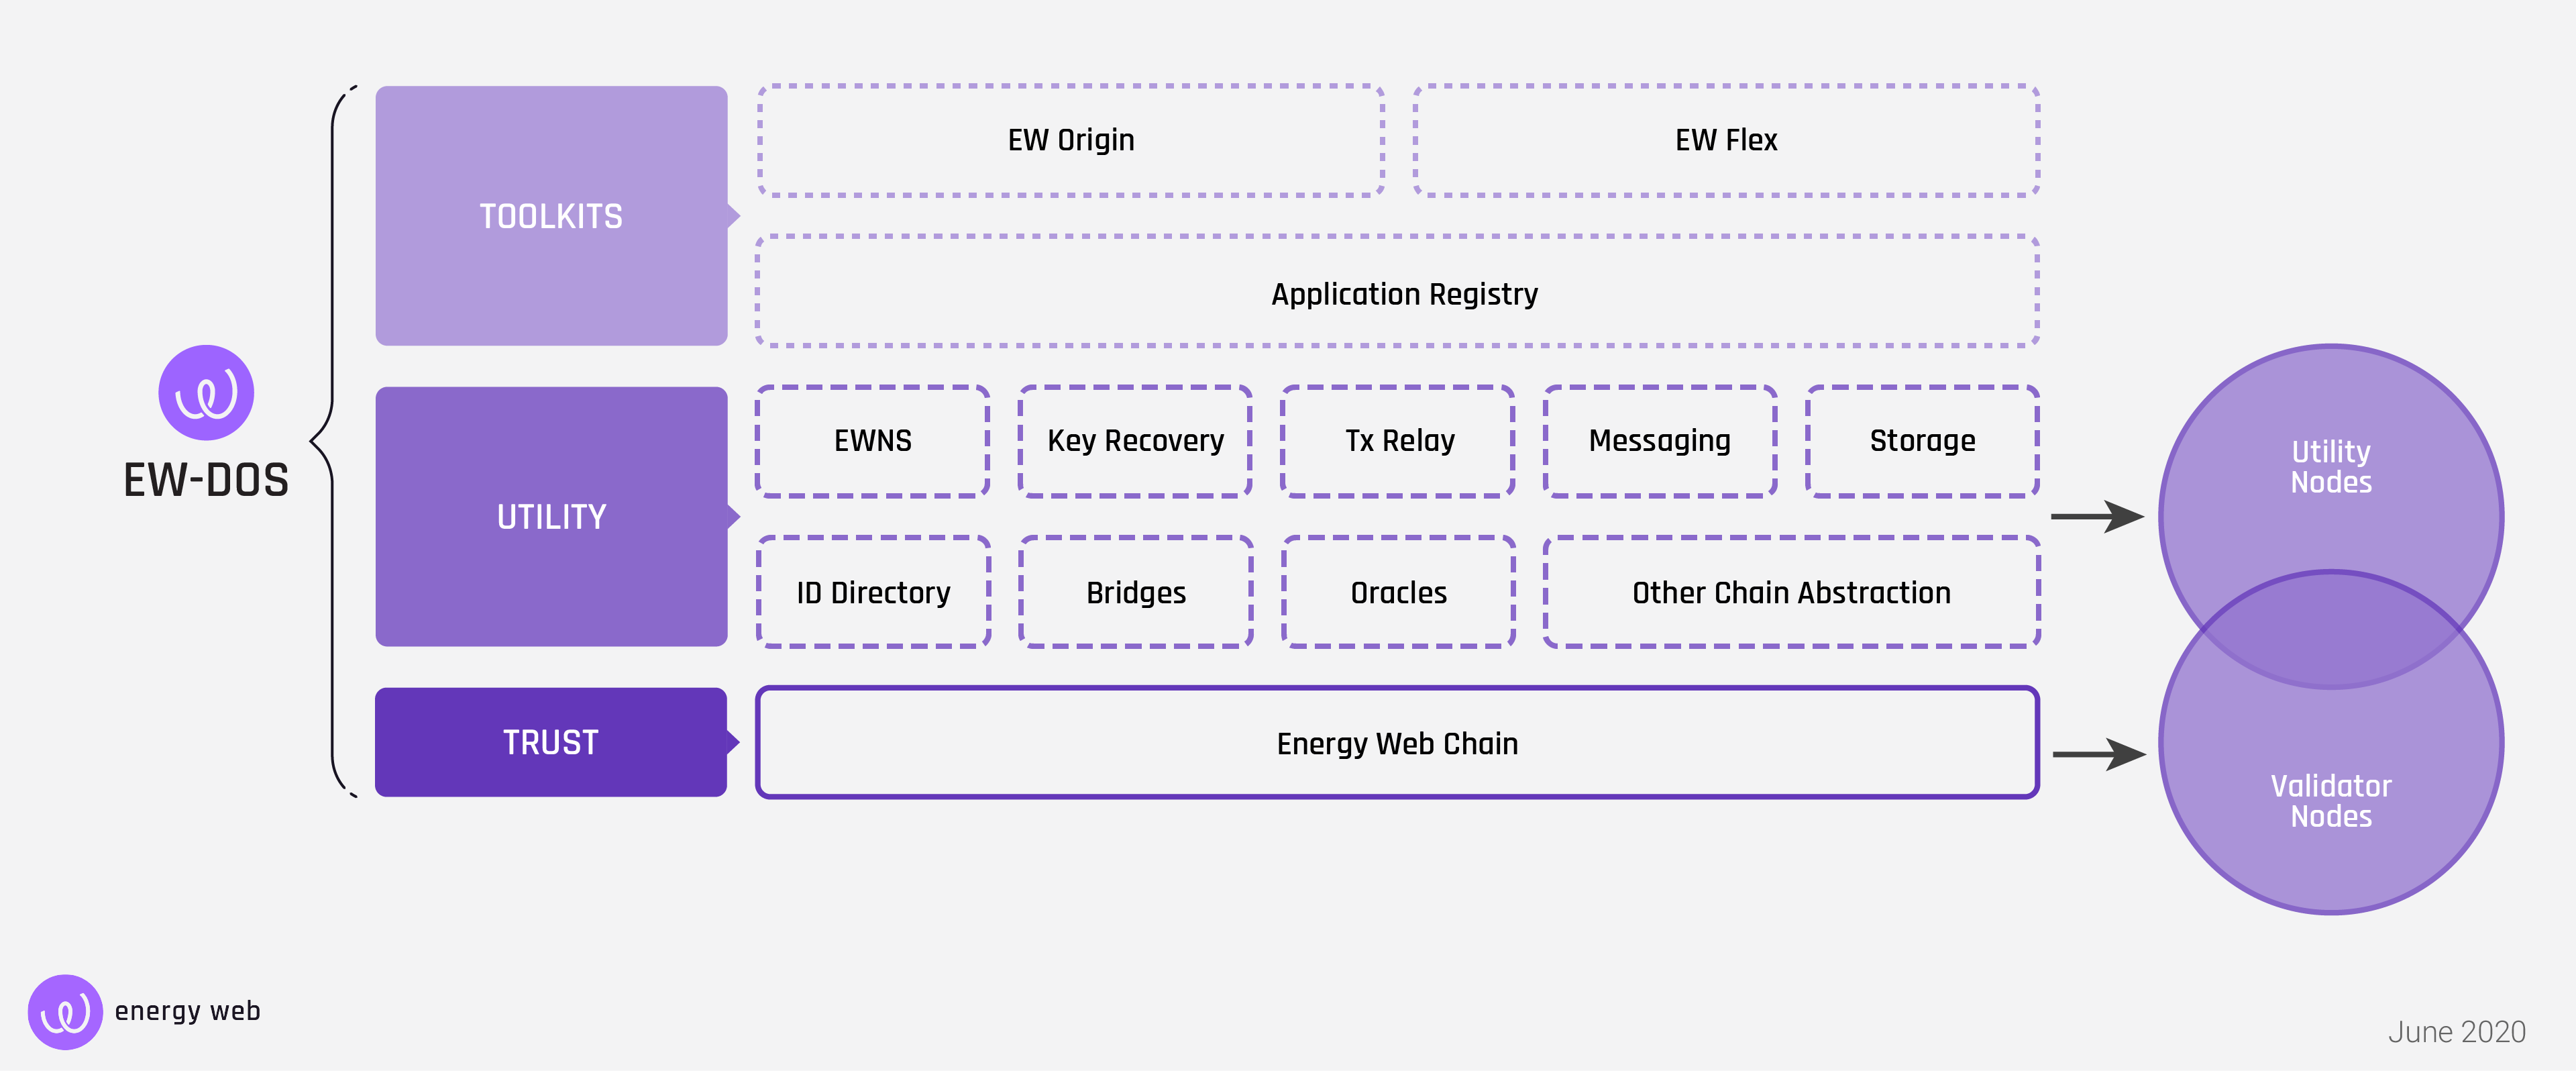
\includegraphics[width=13cm]{ew-dos.png}
    \centering
    \label{ew-dos}
    \caption{Visualizzazione della struttura di EW-DOS \cite{img:ew-dos}}
\end{figure}

\newpage

\section{Differenze con Ethereum}
Non è un mistero che la \gls{ewc} sia molto ispirata ad Ethereum.
Alcuni dei servizi offerti, come l'\gls{ewns} sono fork con modifiche minime di progetti nati su Ethereum. \\
Tuttavia, ci sono alcuni aspetti e funzionalità che hanno necessitato una revisione più profonda, per evitare ostacolassero la visione dietro il progetto. \\

\begin{tabular}{||p{7cm}|p{7cm}||}
    \hline
    Problema                                                    & Modifica                                                                                \\
    \hline\hline
    Basso throughput, alti costi, scalabilità limitata          & Utilizzo della \gls{poa}. Incrementa il throughput fino a 30x                           \\
    \hline
    Poco adatta a piccoli dispositivi (IoT)                     & Maggiore focus sui \textbf{light client} per connettere anche piccoli dispositivi (IoT) \\
    \hline
    Nessuna distinzione fra i nodi con diverse autorizzazioni   & È possibile differenziare fra nodi con compiti ed autorizzazioni diverse                \\
    \hline
    Difficoltà a gestire transazioni che necessitino di privacy & Possibilità di mantenere i dati privati, se richiesto                                   \\[1ex]
    \hline
\end{tabular}

\newpage

\section{Testnet}
Energy Web mette ovviamente a disposizione una testnet che permette a chiunque sia interessato alle peculiarità della loro offerta di testare tutti i servizi senza spendere nulla. \\
La testnet si chiama Volta, e non è dissimile alle testnet che affiancano Ethereum. \\

Di seguito il confronto fra Volta e la \gls{ewc}

\begin{tabular}{||p{4cm}|p{5cm} p{5cm}||}
    \hline
                       & Volta                                               & EWC                                                     \\ [0.5ex]
    \hline\hline
    Data di lancio     & Aprile 2019                                         & Giugno 2019                                             \\
    \hline
    Funzione primaria  & Pre-produzione                                      & Produzione                                              \\
    \hline
    Token              & 90M + 10M di compensi \newline transazioni e faucet & 90M + 10M di compensi \newline transazioni              \\
    \hline
    Tariffe            & Le risorse usate non hanno valore monetario         & Valore monetario delle transazioni in base al gas usato \\
    \hline
    caratteristiche    & 5 secondi per block \newline limite di 8M gas       & 5 secondi per block \newline limite di 8M gas           \\
    \hline
    Connessione ad ETH & Kovan Test Net                                      & ERC-20 token                                            \\
    \hline
    Nodi validatori    & 3 al lancio \newline max 150                        & 10 al lancio \newline max 150                           \\ [1ex]
    \hline
\end{tabular}

\newpage

\section{Algoritmo di consenso \gls{poa}}
L'algoritmo che permette di assicurare un consenso sullo stato della blockchain fra tutti i nodi è \gls{poa}, più precisamente l'algoritmo Aura \cite{art:aura}\cite{wiki:poa}. \\
Nel caso di \gls{ewc}, i validatori sono i partner dell'associazione.
Si tratta, nella maggior parte dei casi, di aziende leader del settore energetico. \\
In breve, il funzionamento è il seguente:

\begin{itemize}
    \item Tutti i nodi validatori possiedono una lista aggiornata degli altri nodi validatori, oltre alla copia completa della blockchain e ad alcuni meta-dati ad essa collegati (es. il throughput della blockchain)
    \item Per una finestra temporale ben definita, un validatore primario viene scelto dall'algoritmo e svolge il compito di raccogliere le transazioni e produrre il nuovo block. La scelta del validatore primario è in funzione del timestamp e del numero di validatori
    \item Se il validatore primario non riesce a produrre il block (es. problemi hardware) o il blocco non viene convalidato dagli altri nodi (es. problemi di connessione), il prossimo validatore primario riprenderà dalle transazioni rimaste in sospeso
    \item Gli altri validatori controllano che le transazioni siano legittime e firmano il block per poi propagarlo alla rete
    \item Se la maggior parte dei validatori hanno verificato il blocco, questo è aggiunto alla blockchain
\end{itemize}

\newpage

\begin{figure}[!h]
    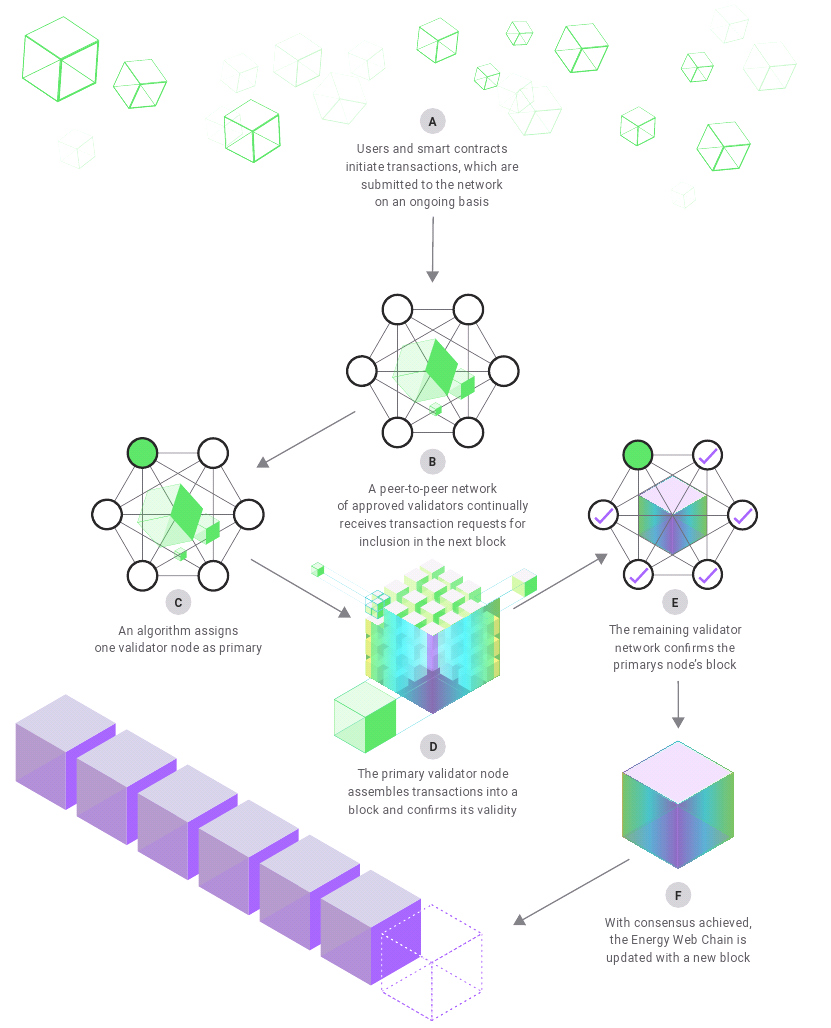
\includegraphics[height=14cm,keepaspectratio]{ew-poa.jpg}
    \centering
    \label{ew-poa}
    \caption{Passi dell'algoritmo \gls{poa} \cite{img:ew-poa}}
\end{figure}

\newpage

\section{Costi di transazione}
Una transazione è una qualsiasi operazione che modifica lo stato della blockchain. Trasferire token fra account, creare un nuovo smart contract o modificarne lo stato sono esempi di transazioni. \\
Il costo da pagare per poter effettuare una transazione dipende dai seguenti fattori:

\begin{itemize}
    \item \textbf{Il costo in gas:} il gas rappresenta la complessità computazionale necessaria per risolvere la transazione. Più è complessa l'operazione più gas sarà richiesto
    \item \textbf{Prezzo del gas:} valore dell'unità di gas in EWT. Prima di effettuare una transazione, l'utente stabilisce quanto è disposto a pagare per unità di gas. Più è alta l'offerta, maggiore sarà la priorità della transazione
    \item \textbf{Valore di mercato del token:} se si vuole ottenere il costo della transazioni in moneta fiat, basta effettuare la conversione fra EWT spesi e il loro valore monetario
\end{itemize}

Riassumendo con una formula: \\
$ costo(\$) = costo\ gas(gas) * prezzo\ gas(token/gas) * valore\ token (\$/token) $. \\

\newpage

\section{Transazioni private}
Una delle caratteristiche fondanti di ogni blockchain è la possibilità di tracciare e verificare ogni transazione che avviene sulla chain. \\
Questa proprietà fondamentale, però, non è sempre desiderabile: anche per ottemperare alle regolamentazioni vigenti riguardanti la privacy, è necessario che ci sia la possibilità di nascondere informazioni sensibili da occhi indiscreti. \\
Sono stati quindi individuati diversi approcci per risolvere il problema. 
Di seguito sono elencati i più promettenti e avanzati.
Per una lista completa è possibile consultare la documentazione \cite{wiki:ew-privacy}

\subsection{Parity Secret Store}
Un'implementazione promettente per risolvere il problema è il Secret Store di del client Parity Ethereum. \\
L'idea è quella di generare una coppia di chiavi, pubblica e privata. 
Quella pubblica è nota, ed è utilizzata per crittografare i messaggi.
Tuttavia, per decriptare i messaggi, è necessaria la chiave privata.
Questa viene distribuita fra $n$ nodi, in modo che per poter accedere alle informazioni protette sia necessario che un numero arbitrario $m$ su $n$ di questi sia favorevole. \\
La tecnica crittografica utilizzata è la "elliptic curve threshold encryption" \cite{art:ecdkg}. \\
L'implementazione è quella di un \gls{kms}, che invece di essere centralizzato è distribuito.
La decentralizzazione elimina il \gls{spf}, in quanto nessun nodo singolo ha accesso all'intera chiave. \\
Il sistema di consenso può sfruttare un sistema di votazione simile a quello usato per la governance. \\
Vi sono, però, vari limiti all'uso di questa tecnica. 
Infatti, è richiesto una setup iniziale fra i nodi interessati, compresa una rete separata per i servizi e le API.
Un numero di nodi attivi deve essere garantito in ogni momento per raggiungere il limite inferiore di votanti.
Infine, attualmente l'implementazione è limitata al client Parity / OpenEthereum.

\subsubsection{Parity Private Transactions}
Continuando a costruire sopra il Parity Secret Store, si può immaginare di generare uno smart contract criptato.
Questo verrebbe poi inserito dentro uno smart contract tradizionale pubblico sulla blockchain. \\
A quel punto, solo gli account autorizzati, con le chiavi necessarie, sono in grado di leggere e modificare lo stato del contratto interno.
La nuova transazione viene eseguita e firmata off-chain, e il nuovo stato, criptato, viene reinserito nella blockchain pubblica.

\begin{figure}[h]
    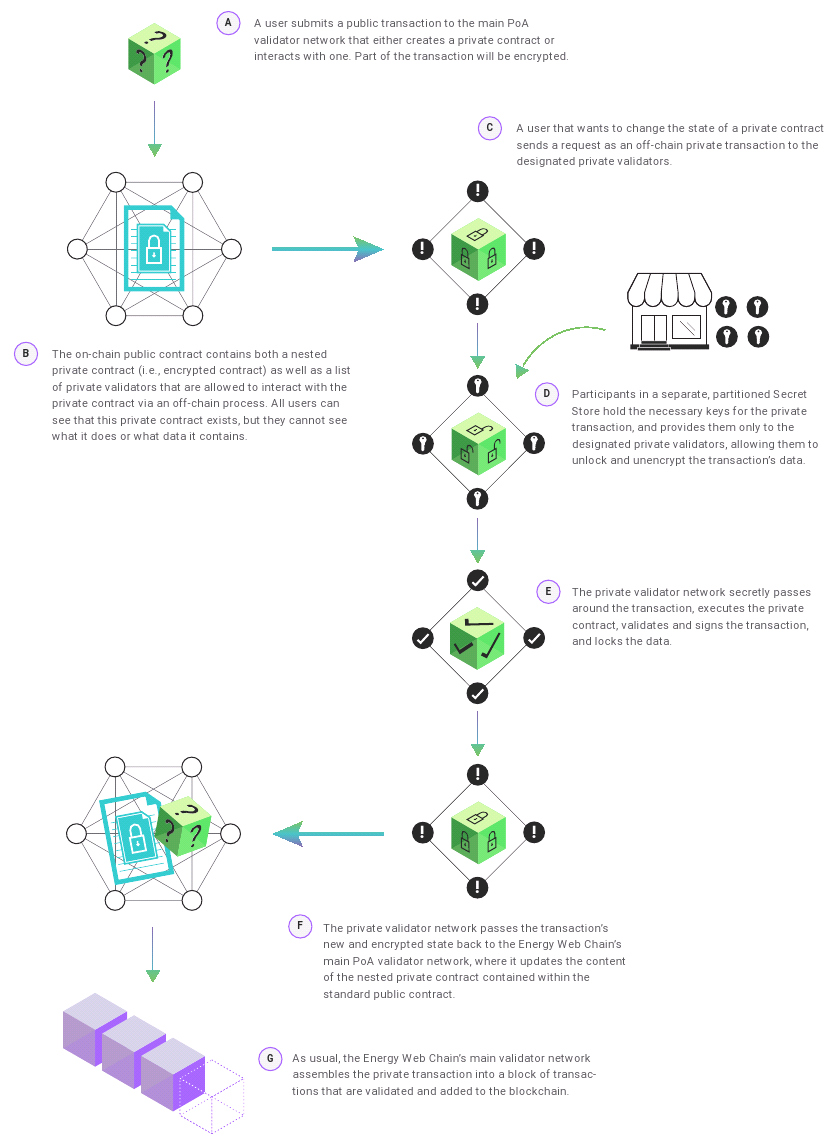
\includegraphics[height=13cm,keepaspectratio]{ew-privacy.jpg}
    \centering
    \label{ew-privacy}
    \caption{Utilizzo di Parity Private Transaction \cite{img:ew-privacy}}
\end{figure}

\subsection{Precise Proofs}
Precise Proofs è uno schema basato sugli alberi di Merkle, in grado di verificare l'autenticità della struttura dati rivelando solo un subset di dati. \\
Si parte realizzando un albero di Merkle a partire dai dati interessati e si rende pubblica la radice. \\
Un terzo ente è interessato a verificare la validità di un subset di dati riceverà solo i dati effettivamente richiesti e le hash dei dati non necessari.
In questo modo si hanno abbastanza informazioni da poter ricostruire la radice minimizzando i dati resi pubblici.

\subsection{Zero Knowledge Proof Protocols}
Gli Zero Knowledge Proof Protocols sono una categoria di protocolli con lo scopo di validare una computazione senza rivelarne alcun input (es. validare una transazione senza rivelare mittente, destinatario, movimento etc.). \\

\subsubsection{zkSNARKs}
zkSNARKs è probabilmente il protocollo più avanzato in questa categoria, sviluppato dal team Zcash. Sebbene sia il più maturo, presenta un tallone d'Achille non indifferente. \\
Per poter utilizzare la Zero Knowledge Proof è necessario realizzare un circuito aritmetico che rappresenta la computazione da provare e generare da quello una coppia di chiavi prover/verifier.
La creazione di questo setup deve essere sicura e pattuita a priori, perché se dovesse essere compromesso un avversario potrebbe approfittarne per realizzare prove false.

\newpage

\section{Storage}
Il fatto che tutti i dati siano immagazzinati sulla blockchain per essere accessibili si traduce in un incremento spesso più che lineare della memoria necessaria per salvare l'intera blockchain su un dispositivo fisico, cosa decisamente non auspicabile se si vuole favorire la partecipazione anche di piccoli dispositivi (IoT). \\
Una prima soluzione è di evitare di immettere dati sulla blockchain, e limitarsi ad utilizzare gli hash degli stessi, per poi poter verificarne la validità off-chain. \\
Nei casi in cui questo non fosse possibile, si può provare ad optare per una delle tante soluzioni che offrono un servizio di storage distribuito.
Le principali soluzioni sono IPFS Storj.
Per una lista completa è possibile consultare la documentazione \cite{wiki:ew-storage}

\subsubsection{\gls{ipfs}}
\gls{ipfs} è un modello di filesystem distribuito.
Invece di indirizzare i file con la loro locazione, li si identifica con un hash ottenuto dal loro contenuto.
Se il file è troppo grande, lo si spezza in più parti con lo stesso risultato. \\
I nodi che fanno parte di questa rete si auto iscrivono in delle tabelle di \gls{dht} che tengono traccia dei nodi che possiedono il file associato ad uno specifico hash. \\
Se si vuole contribuire alla rete, una volta scaricato il file lo si tiene in cache, fornendo ad altri utenti che lo richiedano. \\
Il fatto che un file sia identificato dal suo hash garantisce inoltre l'integrità del dato e la sua immutabilità.
Per aggiornare un file, infatti, bisogna utilizzare il sistema di versioning previsto dal protocollo. \\ \\
Storj è molto simile ad IPFS, con l'incentivo che i nodi sono pagati per svolgere la loro funzione di content-storage.
Ovviamente il contratto prevede che l'host sia in grado fornire su richiesta in qualsiasi momento tutti i file che afferma di possedere.

\newpage

\section{Governance}
La natura decentralizzata della blockchain rende un qualsiasi cambiamento che riguarda la sua infrastruttura un problema non banale. \\
Per gestire al meglio i possibili aggiornamenti che la \gls{ewc} potrebbe necessitare, si è deciso di affidarsi a chi la comprende bene, cioè gli sviluppatori.
Il diritto di voto che determina quali proposte di modifica vengano accolte e quali respinte sarà determinato dalla quantità di gas che un singolo sviluppatore riesce a "generare" con i propri smart contracts.
L'idea è che il valore che lo sviluppatore fornisce all'intero sistema rappresenta il suo peso nella votazione. \cite{wiki:ew-governance} \\
Ciò non esclude che, in caso si renda necessario, alcune scelte troppo complesse possano essere prese da persone designate senza passare per il meccanismo di voto della blockchain.

\begin{figure}[!h]
    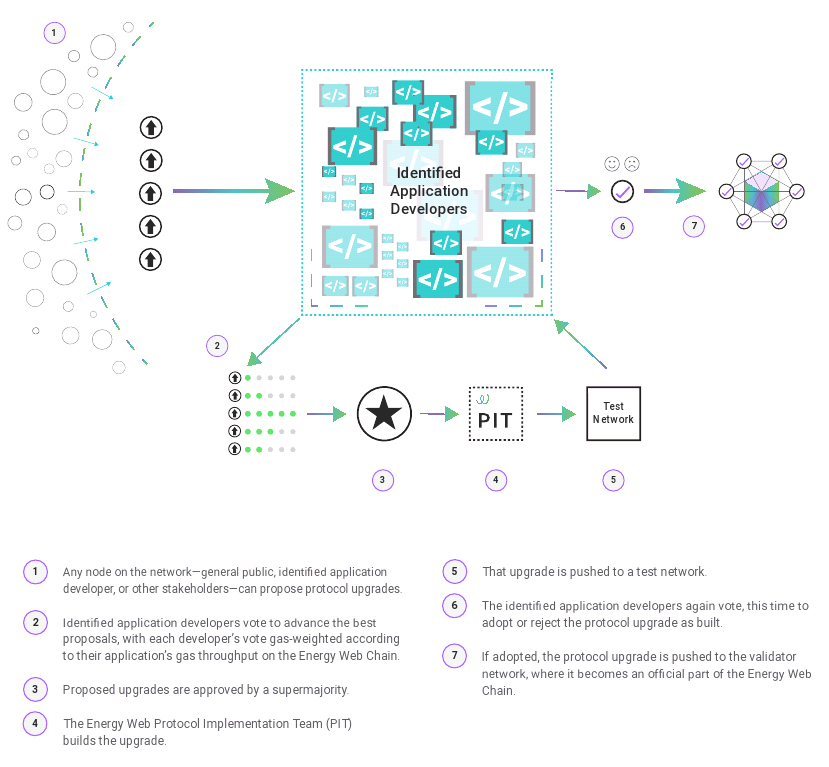
\includegraphics[height=10cm,keepaspectratio]{ew-governance.jpg}
    \centering
    \label{ew-governance}
    \caption{Passi per l'approvazione di una modifica all'infrastruttura di \gls{ewc} \cite{img:ew-governance}}
\end{figure}

\newpage

\section{Staking}
Per fornire quello che nell'architettura di ES-DOS è chiamato "Utility layer", è necessario il contributo di operatori che mettano a disposizione le proprie risorse a chi ha intenzione di sviluppare un servizio.
Perché il tutto sia affidabile e adatto ad un ambiente di produzione, devono essere garantiti dei livelli di servizio, in maniera analoga ad un qualsiasi \gls{sla} proposto da un fornitore di SaaS. \\
La soluzione proposta non è dissimile a quella implementata in altre blockchain, e si rifà al modello \gls{pos}.
Gli attori in questo modello vengono suddivisi in due categorie:

\begin{itemize}
    \item \textbf{Service providers:} sono organizzazioni che mettono a disposizione i nodi di utility. 
    Per essere approvato, un service provider deve poter dimostrare la propria identità e depositare in garanzia una quantità di EWT per un periodo multi-annale.
    Dopo essere stati approvati, i service providers possono aggiungere ulteriori nodi di utility incrementando proporzionalmente il deposito di EWT.
    Finché il \gls{sla} continua ad essere rispettato, i service providers guadagneranno un interesse in base al loro deposito.
    In questo momento, il deposito minimo necessario per essere approvati come service provider si attesta fra i $10000$ e i $100000$ EWT, a cui si aggiungono fra i $1000$ e i $10000$ EWT per service node \cite{art:ew-staking}.
    \item \textbf{Patrons:} sono gli individui o le organizzazioni che finanziano un service provider depositando dei loro EWT per il service provider.
    Differentemente rispetto a ciò che accade per i service provider, non c'è un minimo alla somma depositata e questa può essere ritirata in qualsiasi momento.
    Questo porta i patrons a favorire service provider che rispettano i \gls{sla} e che offrano il miglior modello di revenue-sharing.
\end{itemize}

\begin{figure}[!h]
    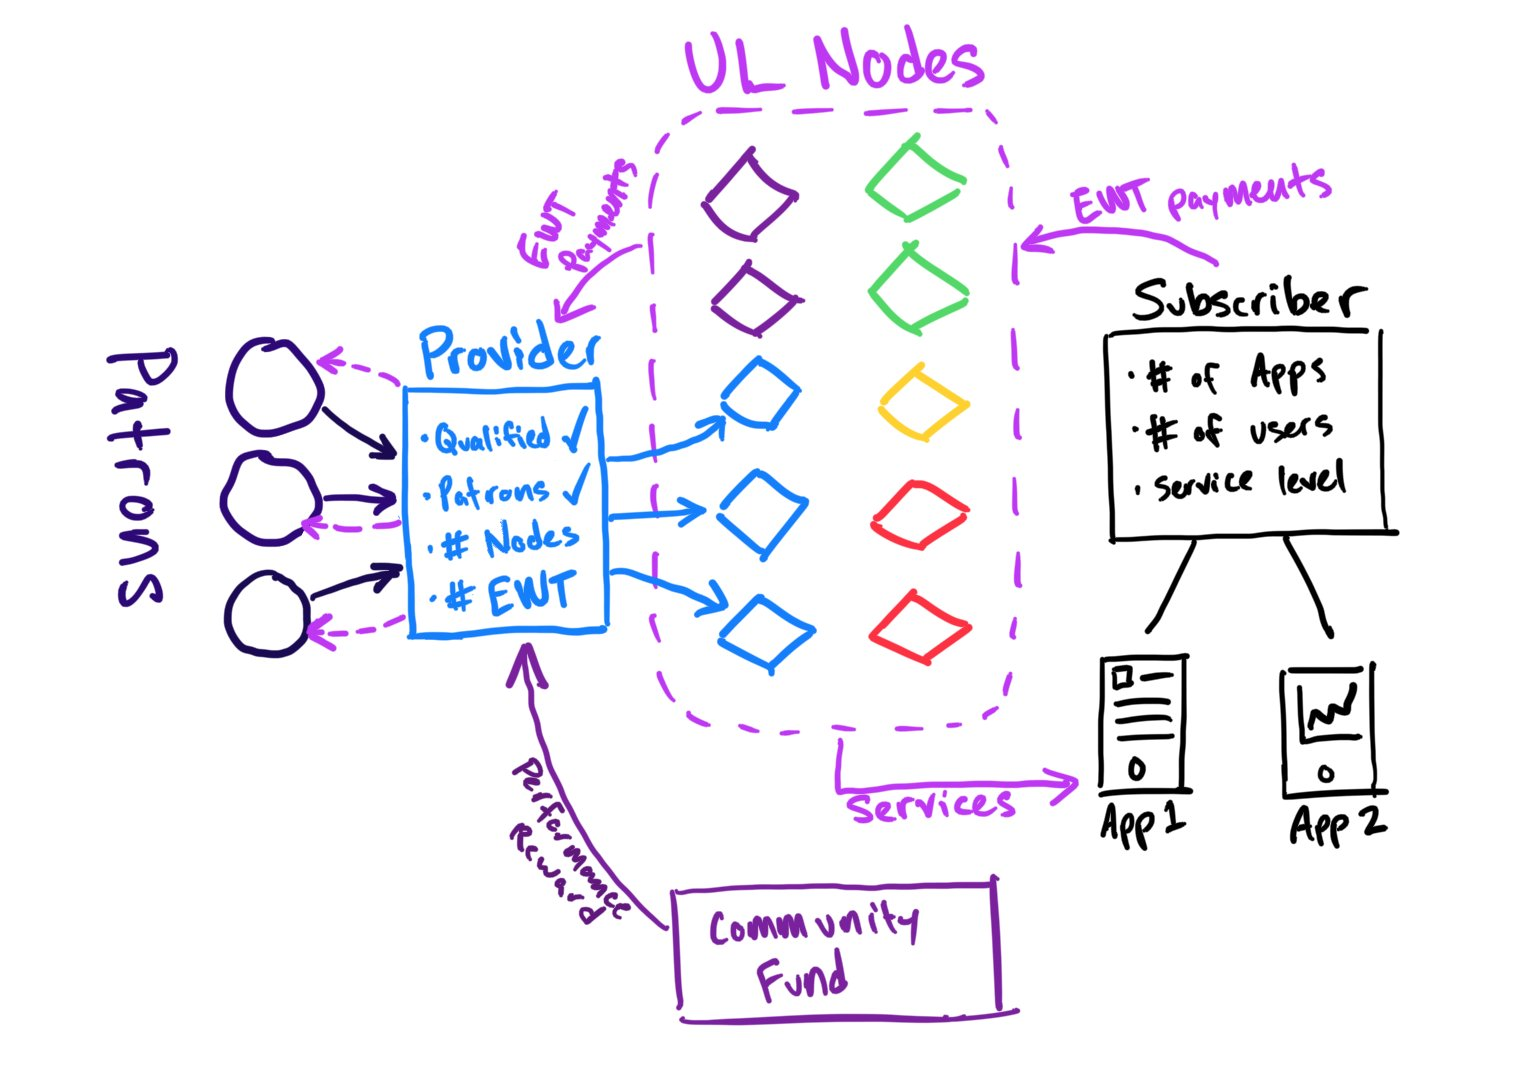
\includegraphics[height=10cm,keepaspectratio]{ew-staking.png}
    \centering
    \label{ew-staking}
    \caption{Come l'utility layer supportato dallo staking si integra in EW-DOS \cite{art:ew-staking}}
\end{figure}

\newpage

\printbibliography
\end{document}
